\documentclass{article}
\usepackage{amsmath}
\usepackage{amssymb}
\usepackage{graphicx}
\usepackage{tikz}
\usepackage{tcolorbox}
\usepackage{xcolor}
\usepackage{algorithm}
\usepackage{algpseudocode}
\usepackage{hyperref}

\title{4. Reinforcement Learning Notes: Policy Iteration}
\author{Rahul Sawhney}

\begin{document}

\maketitle

\tableofcontents
\newpage

\section{Introduction to Policy Iteration}

Policy iteration is a method for finding an optimal policy in a Markov Decision Process (MDP). It works by alternating between two main steps:
\begin{enumerate}
    \item \textbf{Policy Evaluation:} Computing the state-value function $v_\pi$ for a given policy $\pi$.
    \item \textbf{Policy Improvement:} Improving the policy by making it greedy with respect to the current value function.
\end{enumerate}

This process continues until the policy converges to an optimal policy, denoted as $\pi^*$. Policy iteration is at the core of many reinforcement learning methods as it provides a fundamental approach to solving MDPs when the model (transition probabilities and rewards) is known.

\section{Value Functions}

\subsection{State-Value Function}

The state-value function $v_\pi(s)$ represents how good it is for an agent to be in a particular state $s$ when following a policy $\pi$. Formally, it is defined as the expected return (expected cumulative discounted reward) when starting in state $s$ and following policy $\pi$ thereafter:

\begin{equation}
v_\pi(s) \doteq \mathbb{E}_\pi[G_t|S_t = s]
\end{equation}

\begin{tcolorbox}[colframe=blue!50!black, colback=blue!10, title=Notation Overview]
\begin{itemize}
    \item $v_\pi(s)$: State-value function for state $s$ under policy $\pi$
    \item $\mathbb{E}_\pi$: Expected value when following policy $\pi$
    \item $G_t$: Return (cumulative discounted reward) starting from time step $t$
    \item $S_t$: State at time step $t$
    \item $\doteq$: Defined as (definitional equality)
\end{itemize}
\end{tcolorbox}

Utilizing the recursive property of the return, we can also express this as:

\begin{equation}
v_\pi(s) = \mathbb{E}_\pi[R_{t+1} + \gamma G_{t+1}|S_t = s]
\end{equation}

\begin{tcolorbox}[colframe=blue!50!black, colback=blue!10, title=Notation Overview]
\begin{itemize}
    \item $v_\pi(s)$: State-value function for state $s$ under policy $\pi$
    \item $\mathbb{E}_\pi$: Expected value when following policy $\pi$
    \item $R_{t+1}$: Reward received after taking action in state $S_t$
    \item $\gamma$: Discount factor, $0 \leq \gamma \leq 1$, determines the present value of future rewards
    \item $G_{t+1}$: Return starting from time step $t+1$
    \item $S_t$: State at time step $t$
\end{itemize}
\end{tcolorbox}

\subsection{Action-Value Function}

The action-value function $q_\pi(s,a)$ represents how good it is for an agent to take a specific action $a$ in state $s$ and then follow policy $\pi$ thereafter. Formally, it is defined as:

\begin{equation}
q_\pi(s,a) \doteq \mathbb{E}_\pi[G_t|S_t = s, A_t = a]
\end{equation}

\begin{tcolorbox}[colframe=blue!50!black, colback=blue!10, title=Notation Overview]
\begin{itemize}
    \item $q_\pi(s,a)$: Action-value function for taking action $a$ in state $s$ under policy $\pi$
    \item $\mathbb{E}_\pi$: Expected value when following policy $\pi$
    \item $G_t$: Return (cumulative discounted reward) starting from time step $t$
    \item $S_t$: State at time step $t$
    \item $A_t$: Action taken at time step $t$
\end{itemize}
\end{tcolorbox}

\subsection{Bellman Equations for Value Functions}

The Bellman equations provide a recursive definition of value functions, establishing a fundamental relationship between the value of a state and the values of its successor states.

For the state-value function, the Bellman equation is:

\begin{equation}
v_\pi(s) = \sum_a \pi(a|s) \sum_{s',r} p(s',r|s,a)[r + \gamma v_\pi(s')]
\end{equation}

\begin{tcolorbox}[colframe=blue!50!black, colback=blue!10, title=Notation Overview]
\begin{itemize}
    \item $v_\pi(s)$: State-value function for state $s$ under policy $\pi$
    \item $\pi(a|s)$: Probability of taking action $a$ in state $s$ under policy $\pi$
    \item $p(s',r|s,a)$: Probability of transitioning to state $s'$ and receiving reward $r$ when taking action $a$ in state $s$
    \item $\gamma$: Discount factor
    \item $s'$: Next state
    \item $r$: Reward
\end{itemize}
\end{tcolorbox}

For the action-value function, the Bellman equation is:

\begin{equation}
q_\pi(s,a) = \sum_{s',r} p(s',r|s,a)[r + \gamma \sum_{a'} \pi(a'|s')q_\pi(s',a')]
\end{equation}

\begin{tcolorbox}[colframe=blue!50!black, colback=blue!10, title=Notation Overview]
\begin{itemize}
    \item $q_\pi(s,a)$: Action-value function for taking action $a$ in state $s$ under policy $\pi$
    \item $p(s',r|s,a)$: Probability of transitioning to state $s'$ and receiving reward $r$ when taking action $a$ in state $s$
    \item $\pi(a'|s')$: Probability of taking action $a'$ in state $s'$ under policy $\pi$
    \item $\gamma$: Discount factor
    \item $s'$: Next state
    \item $r$: Reward
    \item $a'$: Next action
\end{itemize}
\end{tcolorbox}

\subsection{Relationship Between Value Functions}

The state-value function and action-value function are closely related. The relationship can be expressed as:

\begin{equation}
v_\pi(s) = \sum_a \pi(a|s) q_\pi(s,a)
\end{equation}

\begin{tcolorbox}[colframe=blue!50!black, colback=blue!10, title=Notation Overview]
\begin{itemize}
    \item $v_\pi(s)$: State-value function for state $s$ under policy $\pi$
    \item $q_\pi(s,a)$: Action-value function for taking action $a$ in state $s$ under policy $\pi$
    \item $\pi(a|s)$: Probability of taking action $a$ in state $s$ under policy $\pi$
\end{itemize}
\end{tcolorbox}

And conversely:

\begin{equation}
q_\pi(s,a) = \sum_{s',r} p(s',r|s,a)[r + \gamma v_\pi(s')]
\end{equation}

\begin{tcolorbox}[colframe=blue!50!black, colback=blue!10, title=Notation Overview]
\begin{itemize}
    \item $q_\pi(s,a)$: Action-value function for taking action $a$ in state $s$ under policy $\pi$
    \item $p(s',r|s,a)$: Probability of transitioning to state $s'$ and receiving reward $r$ when taking action $a$ in state $s$
    \item $\gamma$: Discount factor
    \item $v_\pi(s')$: State-value function for state $s'$ under policy $\pi$
    \item $s'$: Next state
    \item $r$: Reward
\end{itemize}
\end{tcolorbox}

\section{Optimal Value Functions}

\subsection{Definitions and Properties}

An optimal policy is a policy that achieves the maximum possible expected return from all states. The optimal state-value function, denoted as $v_*(s)$, gives the maximum value achievable for each state:

\begin{equation}
v_*(s) \doteq \max_\pi v_\pi(s)
\end{equation}

\begin{tcolorbox}[colframe=blue!50!black, colback=blue!10, title=Notation Overview]
\begin{itemize}
    \item $v_*(s)$: Optimal state-value function for state $s$
    \item $\max_\pi$: Maximum over all possible policies $\pi$
    \item $v_\pi(s)$: State-value function for state $s$ under policy $\pi$
\end{itemize}
\end{tcolorbox}

Similarly, the optimal action-value function, denoted as $q_*(s,a)$, gives the maximum value achievable for each state-action pair:

\begin{equation}
q_*(s,a) \doteq \max_\pi q_\pi(s,a)
\end{equation}

\begin{tcolorbox}[colframe=blue!50!black, colback=blue!10, title=Notation Overview]
\begin{itemize}
    \item $q_*(s,a)$: Optimal action-value function for taking action $a$ in state $s$
    \item $\max_\pi$: Maximum over all possible policies $\pi$
    \item $q_\pi(s,a)$: Action-value function for taking action $a$ in state $s$ under policy $\pi$
\end{itemize}
\end{tcolorbox}

\subsection{Bellman Optimality Equations}

The Bellman optimality equation for the state-value function is:

\begin{equation}
v_*(s) = \max_a \sum_{s',r} p(s',r|s,a)[r + \gamma v_*(s')]
\end{equation}

\begin{tcolorbox}[colframe=blue!50!black, colback=blue!10, title=Notation Overview]
\begin{itemize}
    \item $v_*(s)$: Optimal state-value function for state $s$
    \item $\max_a$: Maximum over all possible actions $a$
    \item $p(s',r|s,a)$: Probability of transitioning to state $s'$ and receiving reward $r$ when taking action $a$ in state $s$
    \item $\gamma$: Discount factor
    \item $s'$: Next state
    \item $r$: Reward
\end{itemize}
\end{tcolorbox}

The Bellman optimality equation for the action-value function is:

\begin{equation}
q_*(s,a) = \sum_{s',r} p(s',r|s,a)[r + \gamma \max_{a'} q_*(s',a')]
\end{equation}

\begin{tcolorbox}[colframe=blue!50!black, colback=blue!10, title=Notation Overview]
\begin{itemize}
    \item $q_*(s,a)$: Optimal action-value function for taking action $a$ in state $s$
    \item $p(s',r|s,a)$: Probability of transitioning to state $s'$ and receiving reward $r$ when taking action $a$ in state $s$
    \item $\max_{a'}$: Maximum over all possible next actions $a'$
    \item $\gamma$: Discount factor
    \item $s'$: Next state
    \item $r$: Reward
    \item $a'$: Next action
\end{itemize}
\end{tcolorbox}

\subsection{Relationship Between Optimal Value Functions}

The relationship between the optimal state-value function and the optimal action-value function can be expressed as:

\begin{equation}
v_*(s) = \max_a q_*(s,a)
\end{equation}

\begin{tcolorbox}[colframe=blue!50!black, colback=blue!10, title=Notation Overview]
\begin{itemize}
    \item $v_*(s)$: Optimal state-value function for state $s$
    \item $q_*(s,a)$: Optimal action-value function for taking action $a$ in state $s$
    \item $\max_a$: Maximum over all possible actions $a$
\end{itemize}
\end{tcolorbox}

This shows that the optimal value of a state is the maximum of the optimal action-values for that state, which corresponds to taking the best possible action in that state.

\section{Policy Evaluation}

Policy evaluation is the process of computing the state-value function $v_\pi$ for a given policy $\pi$. This is a crucial step in policy iteration.

\subsection{Iterative Policy Evaluation}

The Bellman equation for the state-value function provides a system of linear equations with one equation for each state. For a finite MDP, this system can be solved directly. However, iterative methods are often more practical, especially for large state spaces.

The iterative policy evaluation algorithm updates the value function as follows:

\begin{equation}
v_{k+1}(s) = \sum_a \pi(a|s) \sum_{s',r} p(s',r|s,a)[r + \gamma v_k(s')]
\end{equation}

\begin{tcolorbox}[colframe=blue!50!black, colback=blue!10, title=Notation Overview]
\begin{itemize}
    \item $v_{k+1}(s)$: Estimated state-value of state $s$ after $k+1$ iterations
    \item $v_k(s)$: Estimated state-value of state $s$ after $k$ iterations
    \item $\pi(a|s)$: Probability of taking action $a$ in state $s$ under policy $\pi$
    \item $p(s',r|s,a)$: Probability of transitioning to state $s'$ and receiving reward $r$ when taking action $a$ in state $s$
    \item $\gamma$: Discount factor
    \item $s'$: Next state
    \item $r$: Reward
\end{itemize}
\end{tcolorbox}

This is a form of dynamic programming update, which converges to the true value function $v_\pi$ as the number of iterations approaches infinity.

\subsection{Iterative Policy Evaluation Algorithm}

\begin{algorithm}
\caption{Iterative Policy Evaluation (for estimating $V \approx v_\pi$)}
\begin{algorithmic}[1]
\State \textbf{Input:} A policy $\pi$ to be evaluated
\State \textbf{Parameter:} A small threshold $\theta > 0$ determining the accuracy of estimation
\State Initialize $V(s) = 0$, for all $s \in \mathcal{S}^+$ (except for terminal states where $V(terminal) = 0$)
\Repeat
\State $\Delta \gets 0$
\For{each $s \in \mathcal{S}$}
\State $v \gets V(s)$
\State $V(s) \gets \sum_a \pi(a|s) \sum_{s',r} p(s',r|s,a)[r + \gamma V(s')]$
\State $\Delta \gets \max(\Delta, |v - V(s)|)$
\EndFor
\Until{$\Delta < \theta$}
\State \textbf{return} $V \approx v_\pi$
\end{algorithmic}
\end{algorithm}

\begin{tcolorbox}[colframe=blue!50!black, colback=blue!10, title=Notation Overview]
\begin{itemize}
    \item $V(s)$: Estimated state-value function
    \item $\pi(a|s)$: Probability of taking action $a$ in state $s$ under policy $\pi$
    \item $p(s',r|s,a)$: Probability of transitioning to state $s'$ and receiving reward $r$ when taking action $a$ in state $s$
    \item $\gamma$: Discount factor
    \item $\mathcal{S}$: Set of all non-terminal states
    \item $\mathcal{S}^+$: Set of all states, including terminal states
    \item $\Delta$: Maximum change in value function
    \item $\theta$: Threshold for convergence
\end{itemize}
\end{tcolorbox}

\section{Policy Improvement}

Policy improvement is the process of making a policy better by making it greedy with respect to the current value function.

\subsection{Policy Improvement Theorem}

The policy improvement theorem states that if we have two policies $\pi$ and $\pi'$ such that, for all states $s \in \mathcal{S}$:

\begin{equation}
q_\pi(s, \pi'(s)) \geq v_\pi(s)
\end{equation}

\begin{tcolorbox}[colframe=blue!50!black, colback=blue!10, title=Notation Overview]
\begin{itemize}
    \item $q_\pi(s, \pi'(s))$: Action-value of taking action prescribed by policy $\pi'$ in state $s$, then following policy $\pi$
    \item $v_\pi(s)$: State-value of state $s$ under policy $\pi$
    \item $\pi'(s)$: Action prescribed by policy $\pi'$ in state $s$
    \item $\mathcal{S}$: Set of all non-terminal states
\end{itemize}
\end{tcolorbox}

Then policy $\pi'$ is at least as good as $\pi$, meaning that $v_{\pi'}(s) \geq v_\pi(s)$ for all $s \in \mathcal{S}$. Furthermore, if there exists at least one state where $q_\pi(s, \pi'(s)) > v_\pi(s)$, then $\pi'$ is strictly better than $\pi$ in at least one state.

The proof of this theorem is based on the recursive nature of value functions. If we start from any state $s$ where $q_\pi(s, \pi'(s)) > v_\pi(s)$, we can show that following $\pi'$ will lead to higher expected returns than following $\pi$.

\subsection{Greedy Policy Improvement}

A natural way to improve a policy is to make it greedy with respect to the current value function. For any deterministic policy $\pi$, the improved policy $\pi'$ is:

\begin{equation}
\pi'(s) = \arg\max_a q_\pi(s,a) = \arg\max_a \sum_{s',r} p(s',r|s,a)[r + \gamma v_\pi(s')]
\end{equation}

\begin{tcolorbox}[colframe=blue!50!black, colback=blue!10, title=Notation Overview]
\begin{itemize}
    \item $\pi'(s)$: Action prescribed by the improved policy in state $s$
    \item $\arg\max_a$: The action $a$ that maximizes the following expression
    \item $q_\pi(s,a)$: Action-value of taking action $a$ in state $s$, then following policy $\pi$
    \item $p(s',r|s,a)$: Probability of transitioning to state $s'$ and receiving reward $r$ when taking action $a$ in state $s$
    \item $\gamma$: Discount factor
    \item $v_\pi(s')$: State-value of state $s'$ under policy $\pi$
\end{itemize}
\end{tcolorbox}

The policy improvement theorem guarantees that this new policy $\pi'$ will be strictly better than $\pi$ unless $\pi$ is already optimal.

\section{Policy Iteration Algorithm}

Policy iteration combines policy evaluation and policy improvement in an iterative process, which converges to an optimal policy.

\begin{algorithm}
\caption{Policy Iteration (for estimating $\pi \approx \pi_*$)}
\begin{algorithmic}[1]
\State \textbf{Initialize:} $V(s) \in \mathbb{R}$ and $\pi(s) \in \mathcal{A}(s)$ arbitrarily for all $s \in \mathcal{S}$
\Repeat
\State // Policy Evaluation
\Repeat
\State $\Delta \gets 0$
\For{each $s \in \mathcal{S}$}
\State $v \gets V(s)$
\State $V(s) \gets \sum_a \pi(a|s) \sum_{s',r} p(s',r|s,a)[r + \gamma V(s')]$
\State $\Delta \gets \max(\Delta, |v - V(s)|)$
\EndFor
\Until{$\Delta < \theta$} (a small positive number determining the accuracy of estimation)
\State // Policy Improvement
\State $\text{policy-stable} \gets \text{true}$
\For{each $s \in \mathcal{S}$}
\State $\text{old-action} \gets \pi(s)$
\State $\pi(s) \gets \arg\max_a \sum_{s',r} p(s',r|s,a)[r + \gamma V(s')]$
\If{$\text{old-action} \neq \pi(s)$}
\State $\text{policy-stable} \gets \text{false}$
\EndIf
\EndFor
\Until{$\text{policy-stable}$}
\State \textbf{return} $V \approx v_*$ and $\pi \approx \pi_*$
\end{algorithmic}
\end{algorithm}

\begin{tcolorbox}[colframe=blue!50!black, colback=blue!10, title=Notation Overview]
\begin{itemize}
    \item $V(s)$: Estimated state-value function
    \item $\pi(s)$: Current policy (deterministic)
    \item $\mathcal{S}$: Set of all non-terminal states
    \item $\mathcal{A}(s)$: Set of actions available in state $s$
    \item $p(s',r|s,a)$: Probability of transitioning to state $s'$ and receiving reward $r$ when taking action $a$ in state $s$
    \item $\gamma$: Discount factor
    \item $\theta$: Threshold for convergence in policy evaluation
    \item $\Delta$: Maximum change in value function
    \item $\text{policy-stable}$: Boolean indicating whether the policy has changed
    \item $\text{old-action}$: Action prescribed by the old policy
    \item $\arg\max_a$: The action $a$ that maximizes the following expression
\end{itemize}
\end{tcolorbox}

\subsection{Convergence of Policy Iteration}

Policy iteration is guaranteed to converge to the optimal policy $\pi_*$ and the optimal value function $v_*$ in a finite number of iterations for any finite MDP. This is because:

\begin{enumerate}
    \item The set of policies for a finite MDP is finite.
    \item Each policy improvement step produces a strictly better policy unless the current policy is already optimal.
    \item Value functions are bounded for finite MDPs with a discount factor $\gamma < 1$.
\end{enumerate}

Therefore, policy iteration must converge to an optimal policy in a finite number of iterations.

\section{Value Iteration}

Value iteration is a variant of policy iteration that combines the policy evaluation and policy improvement steps into a single update. Instead of waiting for policy evaluation to converge completely before policy improvement, value iteration performs a single sweep of policy evaluation followed immediately by policy improvement.

The update rule for value iteration is:

\begin{equation}
v_{k+1}(s) = \max_a \sum_{s',r} p(s',r|s,a)[r + \gamma v_k(s')]
\end{equation}

\begin{tcolorbox}[colframe=blue!50!black, colback=blue!10, title=Notation Overview]
\begin{itemize}
    \item $v_{k+1}(s)$: Estimated state-value of state $s$ after $k+1$ iterations
    \item $v_k(s)$: Estimated state-value of state $s$ after $k$ iterations
    \item $\max_a$: Maximum over all possible actions $a$
    \item $p(s',r|s,a)$: Probability of transitioning to state $s'$ and receiving reward $r$ when taking action $a$ in state $s$
    \item $\gamma$: Discount factor
    \item $s'$: Next state
    \item $r$: Reward
\end{itemize}
\end{tcolorbox}

\begin{algorithm}
\caption{Value Iteration (for estimating $\pi \approx \pi_*$)}
\begin{algorithmic}[1]
\State \textbf{Initialize:} $V(s) = 0$, for all $s \in \mathcal{S}^+$
\Repeat
\State $\Delta \gets 0$
\For{each $s \in \mathcal{S}$}
\State $v \gets V(s)$
\State $V(s) \gets \max_a \sum_{s',r} p(s',r|s,a)[r + \gamma V(s')]$
\State $\Delta \gets \max(\Delta, |v - V(s)|)$
\EndFor
\Until{$\Delta < \theta$} (a small positive number determining the accuracy of estimation)
\State // Output a deterministic policy
\For{each $s \in \mathcal{S}$}
\State $\pi(s) \gets \arg\max_a \sum_{s',r} p(s',r|s,a)[r + \gamma V(s')]$
\EndFor
\State \textbf{return} $\pi \approx \pi_*$
\end{algorithmic}
\end{algorithm}

\begin{tcolorbox}[colframe=blue!50!black, colback=blue!10, title=Notation Overview]
\begin{itemize}
    \item $V(s)$: Estimated state-value function
    \item $\mathcal{S}$: Set of all non-terminal states
    \item $\mathcal{S}^+$: Set of all states, including terminal states
    \item $\max_a$: Maximum over all possible actions $a$
    \item $\arg\max_a$: The action $a$ that maximizes the following expression
    \item $p(s',r|s,a)$: Probability of transitioning to state $s'$ and receiving reward $r$ when taking action $a$ in state $s$
    \item $\gamma$: Discount factor
    \item $\theta$: Threshold for convergence
    \item $\Delta$: Maximum change in value function
    \item $\pi(s)$: Deterministic optimal policy
\end{itemize}
\end{tcolorbox}

\section{Example: Grid World}

Let's consider a simple grid world example to illustrate policy iteration. The grid world is a 4x4 grid with states labeled from (0,0) to (3,3). The agent can move in four directions: up, down, left, and right. If the agent attempts to move off the grid, it remains in the same state. The agent receives a reward of -1 for each move, except when it reaches the goal state (3,3), where it receives a reward of +10 and the episode terminates.

\begin{figure}[h]
\centering
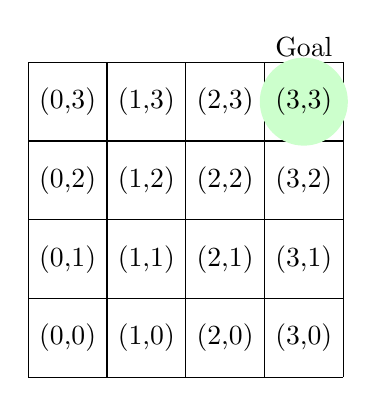
\begin{tikzpicture}[scale=1.0]
    % Grid
    \draw[step=1.0,black,thin] (0,0) grid (4,4);
    
    % State labels
    \node at (0.5,0.5) {(0,0)};
    \node at (1.5,0.5) {(1,0)};
    \node at (2.5,0.5) {(2,0)};
    \node at (3.5,0.5) {(3,0)};
    
    \node at (0.5,1.5) {(0,1)};
    \node at (1.5,1.5) {(1,1)};
    \node at (2.5,1.5) {(2,1)};
    \node at (3.5,1.5) {(3,1)};
    
    \node at (0.5,2.5) {(0,2)};
    \node at (1.5,2.5) {(1,2)};
    \node at (2.5,2.5) {(2,2)};
    \node at (3.5,2.5) {(3,2)};
    
    \node at (0.5,3.5) {(0,3)};
    \node at (1.5,3.5) {(1,3)};
    \node at (2.5,3.5) {(2,3)};
    \node[circle,fill=green!20] at (3.5,3.5) {(3,3)};
    
    % Goal indicator
    \node at (3.5,4.2) {Goal};
\end{tikzpicture}
\caption{4x4 Grid World}
\end{figure}

\subsection{Initial Policy and Value Function}

We start with an arbitrary policy, such as moving right in all states, and initialize the value function to zero for all states (except terminal states).

\subsection{Policy Evaluation}

Using the policy evaluation algorithm, we iteratively update the value function for the current policy. For example, for state (0,0), following the "move right" policy:

\begin{align*}
v_\pi(0,0) &= \sum_a \pi(a|(0,0)) \sum_{s',r} p(s',r|(0,0),a)[r + \gamma v_\pi(s')] \\
&= 1 \cdot \sum_{s',r} p(s',r|(0,0),\text{right})[r + \gamma v_\pi(s')] \\
&= 1 \cdot [(-1) + 0.9 \cdot v_\pi(1,0)]
\end{align*}

Assuming $\gamma = 0.9$, and continuing this process for all states, we eventually converge to the value function for the initial policy.

\subsection{Policy Improvement}

Once we have the value function for the current policy, we improve the policy by making it greedy with respect to the value function:

\begin{align*}
\pi'(s) &= \arg\max_a \sum_{s',r} p(s',r|s,a)[r + \gamma v_\pi(s')]
\end{align*}

For example, for state (0,0), we would consider all four actions (up, down, left, right) and choose the one that gives the highest expected return. After improving the policy for all states, we check if the policy has changed. If it has, we go back to the policy evaluation step with the new policy.

\subsection{Convergence}

We repeat the policy evaluation and policy improvement steps until the policy no longer changes. At this point, we have found an optimal policy for the grid world, which tells the agent the best action to take in each state to maximize the expected return.

\section{Generalized Policy Iteration}

Generalized Policy Iteration (GPI) is a term that refers to the general idea of letting policy evaluation and policy improvement processes interact, regardless of how they are implemented. Most reinforcement learning methods can be viewed as approximations to GPI.

In GPI, the value function is repeatedly pushed toward the value function for the current policy (policy evaluation), while the policy is repeatedly improved with respect to the current value function (policy improvement). These two processes work together, both pushing toward the optimal value function and optimal policy.

\begin{figure}[h]
\centering
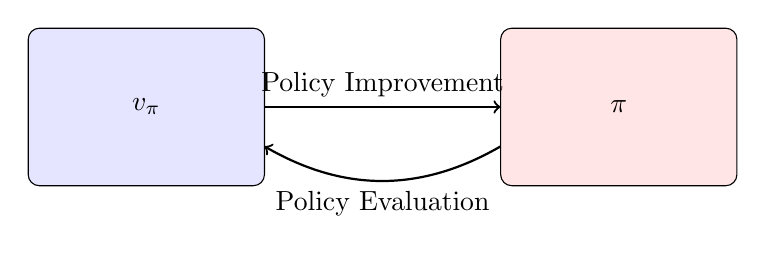
\begin{tikzpicture}
    % Box for value function
    \draw[rounded corners, fill=blue!10] (0,0) rectangle (3,2);
    \node at (1.5,1) {$v_\pi$};
    
    % Box for policy
    \draw[rounded corners, fill=red!10] (6,0) rectangle (9,2);
    \node at (7.5,1) {$\pi$};
    
    % Arrows
    \draw[->, thick] (3,1) -- (6,1) node[midway, above] {Policy Improvement};
    \draw[->, thick, bend left=30] (6,0.5) to node[below] {Policy Evaluation} (3,0.5);
\end{tikzpicture}
\caption{Generalized Policy Iteration}
\end{figure}

\section{Efficiency of Policy Iteration vs Value Iteration}

Both policy iteration and value iteration are guaranteed to converge to an optimal policy, but they have different computational characteristics:

\begin{itemize}
    \item \textbf{Policy Iteration}: Requires fewer iterations but each iteration is more computationally expensive due to the complete policy evaluation step.
    \item \textbf{Value Iteration}: Requires more iterations but each iteration is less computationally expensive due to the single backup operation.
\end{itemize}

In practice, a modified version of policy iteration is often used, where the policy evaluation step is truncated after a fixed number of iterations or when a certain convergence criterion is met. This approach, known as truncated policy iteration, combines the advantages of both policy iteration and value iteration.

\section{Theoretical Guarantees}

Policy iteration is guaranteed to converge to an optimal policy and value function in a finite number of iterations for any finite MDP. This is because:

\begin{enumerate}
    \item The policy improvement step always yields a strictly better policy unless the current policy is already optimal.
    \item There are only a finite number of deterministic policies for a finite MDP.
\end{enumerate}

Similarly, value iteration is also guaranteed to converge to the optimal value function for any finite MDP, as long as the discount factor $\gamma < 1$ (for continuing tasks) or all episodes terminate (for episodic tasks).

\section{Conclusion}

Policy iteration is a fundamental algorithm in reinforcement learning for finding optimal policies in MDPs. It consists of two main steps: policy evaluation, which computes the value function for a given policy, and policy improvement, which makes the policy greedy with respect to the computed value function. The algorithm alternates between these two steps until convergence.

Value iteration is a variant of policy iteration that combines the policy evaluation and policy improvement steps into a single update, often resulting in faster convergence for large state spaces.

Both policy iteration and value iteration are instances of the more general concept of Generalized Policy Iteration (GPI), which forms the foundation of many reinforcement learning algorithms.

When the MDP model (transition probabilities and rewards) is known, policy iteration and value iteration provide powerful tools for solving reinforcement learning problems. However, in many practical scenarios, the model is not known, leading to the development of model-free reinforcement learning methods that estimate value functions directly from experience.

\end{document}
